\documentclass[handout]{beamer}
%\usepackage{beamerthemelined}
\usepackage{pstricks}
\usepackage{amsfonts,amssymb,amsmath,amsthm}
\usepackage{graphicx}
\usepackage[draft]{animate}
\usepackage{wallpaper}
%\setbeamertemplate{navigation symbols}{}
\beamertemplatenavigationsymbolsempty

\usetheme{Boadilla}
\usecolortheme{whale}
\setbeamertemplate{itemize items}[triangle]


\title{Hard Polyhedra Fluids}
\author{Paho Lurie-Gregg}
\date{}

\newcommand{\f}[2]{\dfrac{#1}{#2}}
\newcommand{\p}[1]{\left(#1\right)}
\renewcommand{\t}[1]{\text{#1}}
\newcommand{\abs}[1]{\left|#1\right|}

\begin{document}
{
\usebackgroundtemplate{
\includegraphics[width=\paperwidth]{figs/background}}
\begin{frame}
  \maketitle
 \begin{center}
   Dr. David Roundy, Department of Physics
 \end{center}

\end{frame}
}
\begin{frame}
  \frametitle{Water}
  \begin{itemize}
  \item<1-> Water is arguably the most important fluid in existence, and yet it has some very strange properties
  \item<2-> There currently exist no accurate continuum models for water at melting
  \end{itemize}
  \begin{figure}[h]
    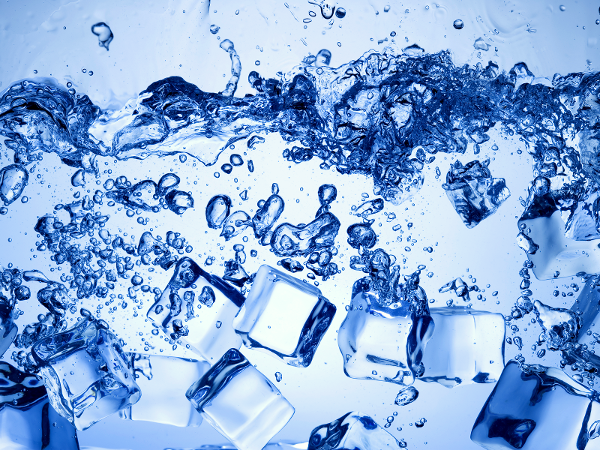
\includegraphics[width=80mm]{figs/ice-water.png}
  \end{figure}
\end{frame}

\begin{frame}
  \frametitle{Background}
  Why Hard Polyhedra?
  \begin{itemize}
  \item<1-> Hard sphere fluids have been studied extensively
  \item<2-> Hard polyhedra have little known theory
  \item<3-> We expect to be able to match the crystal structure of ice with truncated tetrahedra
  \item<4-> Other polyhedra may show interesting characteristics
  \end{itemize}
  \begin{figure}[h]
    \raggedleft
    \includegraphics[width=60mm]{figs/Cryst_struct_ice}
  \end{figure}
\end{frame}
\begin{frame}
  \frametitle{Classical Density Functional Theory}
  \begin{itemize}
  \item<1-> A functional is simply a function of a function
  \item<2-> Classical DFT provides a continuum approach for fluids
  \item<3-> Helmholtz Free Energy is minimized at equilibrium
    \begin{align*}
      F = U - TS
    \end{align*}
  \end{itemize}
\end{frame}


\begin{frame}
  \frametitle{Monte Carlo Example}
  \begin{figure}[h]
    \centering
    \animategraphics[width=100mm,autoplay]{.6}{anim/mc-slow-}{000}{200}
  \end{figure}

\end{frame}

\begin{frame}
  \frametitle{Monte Carlo Example}
  \begin{figure}[h]
    \centering
    \animategraphics[width=120mm,autoplay]{3}{anim/mc100-0.50-}{000}{999}
  \end{figure}

\end{frame}
\end{document}

